% Harus dimuat terlebih dahulu, digunakan agar file PDF memiliki format karakter yang benar.
% Untuk informasi lebih lanjut, lihat https://ctan.org/pkg/cmap.
\RequirePackage{cmap}

% Format dokumen sebagai paper konferensi menggunakan aturan IEEEtran terbaru (v1.8b).
% Untuk informasi lebih lanjut, lihat http://www.michaelshell.org/tex/ieeetran/.
\documentclass[a4paper, conference]{IEEEtran}

% Format encoding font dan input menjadi 8-bit UTF-8.
\usepackage[T1]{fontenc}
\usepackage[utf8]{inputenc}
\usepackage{amsmath}

% Digunakan untuk mengatur margin dokumen.
\usepackage{textcomp}

% Format bahasa menjadi bahasa indonesia dan inggris.
\usepackage[indonesian]{babel}

% Digunakan untuk tujuan demonstrasi.
\usepackage{mwe}

% Digunakan untuk menampilkan font dengan style yang lebih baik.
\usepackage[zerostyle=b,scaled=.75]{newtxtt}

% Digunakan untuk menampilkan tabel dengan style yang lebih baik.
\usepackage{booktabs}
\usepackage[table,xcdraw]{xcolor}
% Digunakan untuk menampilkan gambar pada dokumen.
\usepackage{graphicx}

% Digunakan untuk menampilkan potongan kode.
\usepackage{listings}
\lstset{
  basicstyle=\ttfamily,
  columns=fixed,
  basewidth=.5em,
  xleftmargin=0.5cm,
  captionpos=b
}

\usepackage{tabularx}
\usepackage{wrapfig}
% Digunakan agar backticks (`) dapat dirender pada PDF.
% Untuk informasi lebih lanjut, lihat https://tex.stackexchange.com/a/341057/9075.
\usepackage{upquote}

% Digunakan untuk menyeimbangkan bagian akhir dokumen dengan dua kolom.
\usepackage{balance}

% Kapitalisasi caption tabel
\usepackage{caption}
\captionsetup[table]{
    justification=centering, % Memusatkan caption
    labelsep=newline, % Memisahkan label "TABLE 1" dengan judul dengan baris baru
    textfont={sc}, % Membuat teks menjadi kapital
    labelfont={sc} % Membuat teks menjadi kapital
}


% Digunakan untuk menampilkan pustaka.
\usepackage[square,comma,numbers,sort&compress]{natbib}

% Mengubah format ukuran teks pada natbib.
\renewcommand{\bibfont}{\normalfont\footnotesize}

% Jika melebihi 3 penulis dapat dilakukan linebreakend 
\makeatletter
\newcommand{\linebreakand}{%
  \end{@IEEEauthorhalign}
  \hfill\mbox{}\par
  \mbox{}\hfill\begin{@IEEEauthorhalign}
}
\makeatother

% Menambah nama penulis ketika menggunakan perintah \citet.
% Untuk informasi lebih lanjut, lihat https://tex.stackexchange.com/a/76075/9075.
\usepackage{etoolbox}
\makeatletter
\patchcmd{\NAT@test}{\else \NAT@nm}{\else \NAT@hyper@{\NAT@nm}}{}{}
\makeatother

% Digunakan untuk melakukan linewrap pada pustaka dengan url yang panjang
% jika terdapat hyphens
\usepackage[hyphens]{url}

% Digunakan untuk menambah hyperlink pada referensi.
\usepackage{hyperref}

% Menonaktifkan warna dan bookmark pada hyperref.
\hypersetup{hidelinks,
  colorlinks=true,
  allcolors=black,
  pdfstartview=Fit,
  breaklinks=true
}

% Digunakan untuk membenarkan hyperref pada gambar.
\usepackage[all]{hypcap}

% Digunakan untuk menampilkan beberapa gambar
\usepackage[caption=false,font=footnotesize]{subfig}

\usepackage{stfloats}
% nama
\newcommand{\name}{Moh. Iqbal Fatchurozi}
\newcommand{\authorname}{Fatchurozi, Moh. Iqbal}
\newcommand{\nickname}{Iqbal}
\newcommand{\advisor}{Arief Kurniawan}
\newcommand{\coadvisor}{Eko Mulyanto Yuniarno}

% identitas
\newcommand{\nrp}{5024 20 1009}
\newcommand{\advisornip}{19740907 200212 1 001}
\newcommand{\coadvisornip}{19680601 199512 1 009}
\newcommand{\email}{5024201009@student.its.ac.id}
\newcommand{\advisoremail}{arifku@ee.its.ac.id}
\newcommand{\coadvisoremail}{ekomulyanto@ee.its.ac.id}

% judul
\newcommand{\tatitle}{Judul Paper}
\newcommand{\engtatitle}{Paper Title}

% tempat
\newcommand{\place}{Surabaya}

% jurusan
\newcommand{\studyprogram}{Teknik Komputer}
\newcommand{\engstudyprogram}{Computer Engineering}

% fakultas
\newcommand{\faculty}{Teknologi Elektro dan Informatika Cerdas}
\newcommand{\engfaculty}{Intelligence Electrical and Informatics Technology}

% singkatan fakultas
\newcommand{\facultyshort}{FTEIC}
\newcommand{\engfacultyshort}{ELECTICS}

% departemen
\newcommand{\department}{Teknik Komputer}
\newcommand{\engdepartment}{Computer Engineering}

% Tambahkan format tanda hubung yang benar di sini
\hyphenation{
  ro-ket
  me-ngem-bang-kan
  per-hi-tu-ngan
}


\begin{document}

% Ubah kalimat berikut sesuai dengan judul penelitian.
\title{\tatitle{}}

% Ubah kalimat-kalimat berikut sesuai dengan nama, institusi, alamat dan kontak penulis.
\author{
  \IEEEauthorblockN{\name{}}
  \IEEEauthorblockA{\textit{Departemen \studyprogram{}}\\
    \textit{Institut Teknologi Sepuluh Nopember}\\
    Surabaya, Indonesia 60111\\
    \email{}}

  \and
  \IEEEauthorblockN{\advisor{}}
  \IEEEauthorblockA{\textit{Departemen \studyprogram{}}\\
    \textit{Institut Teknologi Sepuluh Nopember}\\
    Surabaya, Indonesia 60111\\
    \advisoremail{}}

  \and
  \IEEEauthorblockN{\coadvisor{}}
  \IEEEauthorblockA{\textit{Departemen \studyprogram{}}\\
    \textit{Institut Teknologi Sepuluh Nopember}\\
    Surabaya, Indonesia 60111\\
    \coadvisoremail{}}
}

% Digunakan untuk menampilkan judul dan deskripsi penulis.
\maketitle

% Mengubah keterangan `Abstract` ke bahasa indonesia.
% Hapus bagian ini untuk mengembalikan ke format awal.
\renewcommand\abstractname{Abstrak}

\begin{abstract}

  % Ubah paragraf berikut sesuai dengan abstrak dari penelitian.
  Penelitian ini menghadirkan pendekatan baru untuk meningkatkan mobilitas bagi pasien
  ALS dengan mengembangkan sistem kontrol pergerakan kursi roda menggunakan MediaPipe,
  yang berfokus pada pengenalan gerakan mata, dan diimplementasikan pada platform Jetson
  Nano. Studi ini didorong oleh tantangan yang dihadapi oleh pasien ALS, yang meskipun
  kehilangan mobilitas fisik, tetap dapat menggerakkan mata. Sistem yang diusulkan bertujuan
  untuk memberikan kemandirian yang lebih besar dan peningkatan kualitas hidup bagi individu
  tersebut. Metodologi penelitian ini terdiri dari beberapa komponen kunci: pengambilan dan
  pengolahan gambar mata, ekstraksi fitur yang relevan, estimasi dan klasifikasi posisi mata, serta
  eksekusi sistem kontrol pada Next Unit of Computing (NUC). Integrasi teknologi visi komputer
  dengan sistem tertanam merupakan batu penjuru penelitian ini, memastikan mekanisme kontrol
  kursi roda yang responsif dan efisien. Dengan memanfaatkan kekuatan MediaPipe untuk
  pengenalan gestur waktu nyata dan kemampuan komputasi Jetson Nano, studi ini menjanjikan
  peningkatan yang signifikan dalam otonomi pengguna kursi roda dengan gangguan mobilitas.
  Penelitian ini tidak hanya berkontribusi pada bidang teknologi bantu, tetapi juga berpotensi
  menjadi model untuk inovasi masa depan dalam solusi mobilitas bagi individu dengan berbagai
  disabilitas fisik.

\end{abstract}

% Mengubah keterangan `Index terms` ke bahasa indonesia.
% Hapus bagian ini untuk mengembalikan ke format awal.
\renewcommand\IEEEkeywordsname{Kata kunci}

\begin{IEEEkeywords}

  % Ubah kata-kata berikut sesuai dengan kata kunci dari penelitian.
  Teknologi Bantu, Pengenalan Gerakan, Kontrol Kursi Roda

\end{IEEEkeywords}


% Ubah bagian berikut sesuai dengan konten-konten yang akan dimasukkan pada dokumen
% Ubah judul dan label berikut sesuai dengan yang diinginkan.
\section{Pendahuluan}
\label{sec:pendahuluan}

% Ubah paragraf-paragraf pada bagian ini sesuai dengan yang diinginkan.

\lipsum[1]
% Ubah judul dan label berikut sesuai dengan yang diinginkan.
\section{Tinjauan Pustaka}
\label{sec:tinjauanpustaka}

Beberapa penelitian lain pernah dilakukan seperti yang dirumuskan oleh \citet{newton1687} bahwa \lipsum[5]
Hasil tersebut kemudian menjadi persamaan \ref{eq:hukumpertama}.

% Contoh pembuatan persamaan ilmiah.
\begin{equation}
  \label{eq:hukumpertama}
  \sum \mathbf{F} = 0\; \Leftrightarrow\; \frac{\mathrm{d} \mathbf{v} }{\mathrm{d}t} = 0.
\end{equation}

\lipsum[6-7]
% Ubah judul dan label berikut sesuai dengan yang diinginkan.
\section{Desain dan Implementasi}
\label{sec:desaindanimplementasi}

\subsection{Cetak Biru Roket}
\label{subsec:cetakbiruroket}

Pada cetak biru yang tertera pada Gambar \ref{fig:cetakbiru}. \lipsum[8]

% Contoh input gambar pada kolom.
\lipsum[9-10]

\subsection{Lorem Ipsum}
\label{subsec:loremipsum}

\lipsum[11]

% Contoh pembuatan tabel.
\begin{table}
  \caption{Contoh tabel sederhana}
  \label{tab:tabelsederhana}
  \centering
  \begin{tabular}{lll}
    \toprule
    Heading1 & Heading2 & Heading3 \\
    \midrule
    One      & Two      & Three    \\
    Four     & Five     & Six      \\
    \bottomrule
  \end{tabular}
\end{table}

% Contoh pembuatan potongan kode.
\begin{lstlisting}[
  language=C++,
  caption={Program halo dunia.},
  label={lst:halodunia}
]
#include <iostream>

int main() {
    std::cout << "Halo Dunia!";
    return 0;
}
\end{lstlisting}

\lipsum[12]

% Contoh pembuatan daftar.
\begin{enumerate}
  \item \lipsum[13][1-4]
  \item \lipsum[13][5-8]
  \item \lipsum[13][9-12]
\end{enumerate}

\lipsum[14-15]
% Ubah judul dan label berikut sesuai dengan yang diinginkan.
\section{Hasil dan Pembahasan}
\label{sec:hasildanpembahasan}

% Ubah paragraf-paragraf pada bagian ini sesuai dengan yang diinginkan.
\subsection{Pengujian Performa Model dengan menggunakan Variasi Jarak}

Pada skenario pengujian ini, model diuji berdasarkan beberapa variasi jarak. Pengujian jarak berguna untuk mengetahui performa dan tingkat akurasi model jika input citra diambil dari jarak yang berbeda-beda. Hal ini perlu diuji karena semakin jauh jarak pendeteksi citra, maka semakin kecil data visual citra yang diperoleh. Hasil validasi jarak yang digunakan adalah 30 sentimeter yang dapat dilihat pada Tabel \ref{tb:30cm}, 50 sentimeter pada Tabel \ref{tb:50cm}, 70 sentimeter pada Tabel \ref{tb:70cm}, dan 90 sentimeter pada Tabel \ref{tb:90cm}. Untuk contoh dataset variasi pengujian jarak dapat dilihat pada Gambar \ref{fig:Variasi Jarak Kamera}.

\begin{figure}[H]
  \centering
  \subfloat[30 sentimeter]{
    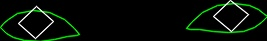
\includegraphics[width=0.2\textwidth]{gambar/bab4/30.jpg}
    %\caption{30 sentimeter}
    \label{fig:imagea}}
    \hfil 
  \subfloat[50 sentimeter]{
    
\includegraphics[width=0.2\textwidth]{gambar/bab4/50.jpg}
    %\caption{50 sentimeter}
    \label{fig:imageb}}

  \subfloat[70 sentimeter]{
    
\includegraphics[width=0.2\textwidth]{gambar/bab4/70.jpg}
    %\caption{70 sentimeter}
    \label{fig:imagec}}
    \hfil
  \subfloat[90 sentimeter]{
    
\includegraphics[width=0.2\textwidth]{gambar/bab4/90.jpg}
    %\caption{90 sentimeter}
    \label{fig:imaged}}

  \caption{Variasi Jarak Kamera}
  \label{fig:Variasi Jarak Kamera}
\end{figure}

\begin{table}[ht]
  \caption{Hasil Validasi Nilai Model dengan Jarak 30 cm}
  \label{tb:30cm}
  \centering
  \begin{tabular}{|l|c|c|c|c|}
  \hline
  \rowcolor[HTML]{C0C0C0} 
  \textbf{Kelas} & \textbf{\emph{Accuracy}} & \textbf{\emph{Precision}} & \textbf{\emph{Recall}} & \textbf{\emph{F1-Score}} \\ \hline
  Kanan    & 100\%            & 100\%             & 100\%           & 100\%            \\ \hline
  Kiri     & 100\%          & 100\%           & 100\%           & 100\%           \\ \hline
  Maju      & 100\%          & 100\%           & 100\%          & 100\%          \\ \hline
  Mundur     & 100\%            & 100\%             & 100\%           & 100\%            \\ \hline
  Stop  & 100\%            & 100\%             & 100\%           & 100\%            \\ \hline
  \end{tabular}
\end{table}

\begin{table}[ht]
  \caption{Hasil Validasi Nilai Model dengan Jarak 50 cm}
  \label{tb:50cm}
  \centering
  \begin{tabular}{|l|c|c|c|c|}
  \hline
  \rowcolor[HTML]{C0C0C0} 
  \textbf{Kelas} & \textbf{\emph{Accuracy}} & \textbf{\emph{Precision}} & \textbf{\emph{Recall}} & \textbf{\emph{F1-Score}} \\ \hline
  Kanan    & 100\%            & 100\%             & 100\%           & 100\%            \\ \hline
  Kiri     & 100\%          & 100\%           & 100\%           & 100\%           \\ \hline
  Maju      & 100\%          & 100\%           & 100\%          & 100\%          \\ \hline
  Mundur     & 100\%            & 100\%             & 100\%           & 100\%            \\ \hline
  Stop  & 100\%            & 100\%             & 100\%           & 100\%            \\ \hline
  \end{tabular}
\end{table}

\begin{table}[ht]
  \caption{Hasil Validasi Nilai Model dengan Jarak 70 cm}
  \label{tb:70cm}
  \centering
  \begin{tabular}{|l|c|c|c|c|}
  \hline
  \rowcolor[HTML]{C0C0C0} 
  \textbf{Kelas} & \textbf{\emph{Accuracy}} & \textbf{\emph{Precision}} & \textbf{\emph{Recall}} & \textbf{\emph{F1-Score}} \\ \hline
  Kanan    & 100\%            & 100\%             & 100\%           & 100\%            \\ \hline
  Kiri     & 100\%          & 100\%           & 100\%           & 100\%           \\ \hline
  Maju      & 99.50\%          & 100\%           & 97.50\%          & 98.73\%          \\ \hline
  Mundur     & 99.50\%            & 97.56\%             & 100\%           & 98.77\%            \\ \hline
  Stop  & 100\%            & 100\%             & 100\%           & 100\%            \\ \hline
  \end{tabular}
\end{table}

\begin{table}[H]
  \caption{Hasil Validasi Nilai Model dengan Jarak 90 cm}
  \label{tb:90cm}
  \centering
  \begin{tabular}{|l|c|c|c|c|}
  \hline
  \rowcolor[HTML]{C0C0C0} 
  \textbf{Kelas} & \textbf{\emph{Accuracy}} & \textbf{\emph{Precision}} & \textbf{\emph{Recall}} & \textbf{\emph{F1-Score}} \\ \hline
  Kanan    & 100\%            & 100\%             & 100\%           & 100\%            \\ \hline
  Kiri     & 100\%          & 100\%           & 100\%           & 100\%           \\ \hline
  Maju      & 96.67\%          & 94.64\%           & 88.33\%          & 91.38\%          \\ \hline
  Mundur     & 96.67\%            & 89.06\%             & 95\%           & 91.94\%            \\ \hline
  Stop  & 100\%            & 100\%             & 100\%           & 100\%            \\ \hline
  \end{tabular}
\end{table}
    
\subsection{Pengujian Performa Model dengan menggunakan Variasi Pencahayaan}

Pada sistem kontrol kursi roda berbasis \emph{gesture} mata, variasi pencahayaan memiliki pengaruh signifikan terhadap performa model deteksi. Tujuan dari pengujian ini adalah untuk mengevaluasi tingkat keberhasilan dan ketidakberhasilan model dalam mendeteksi pose mata pada tiga kondisi pencahayaan \emph{ambient light}, seperti pencahayaan gelap (35 Lux) yang dapat dilihat pada Tabel \ref{tb:lux35}, redup (55 Lux) pada Tabel \ref{tb:lux55}, dan terang (131 Lux) pada Tabel \ref{tb:lux131}. Untuk variasi pengujian pencahayaan dapat dilihat pada Gambar \ref{fig:Variasi Pencahayaan}.

\begin{figure}[H]
  \centering
  \subfloat[35 Lux]{
    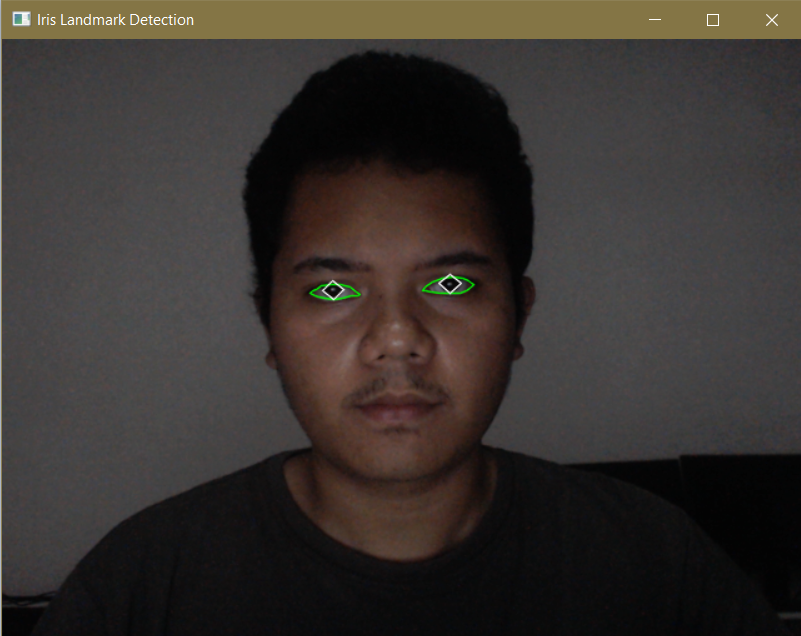
\includegraphics[width=0.15\textwidth]{gambar/bab4/33.png}
    %\caption{30 sentimeter}
    \label{fig:imageaa}}
  \hfil
  \subfloat[55 Lux]{
    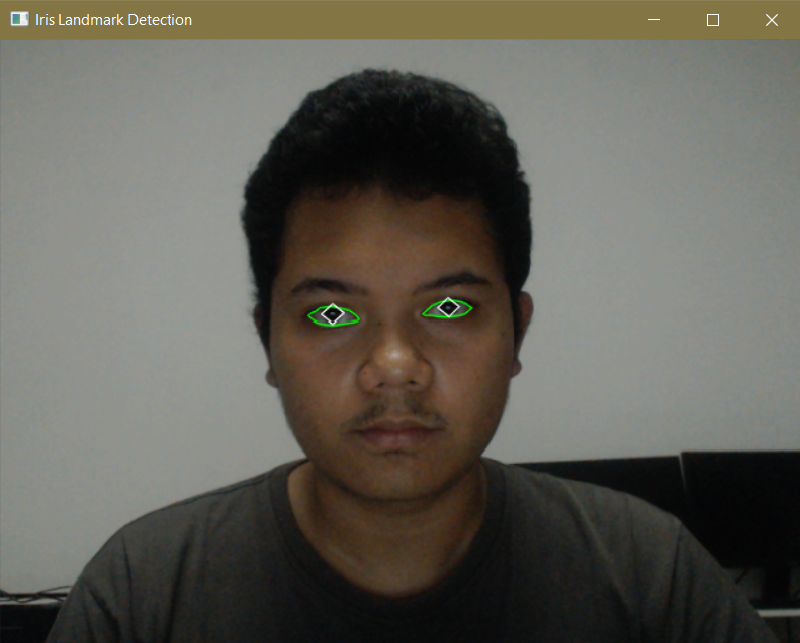
\includegraphics[width=0.15\textwidth]{gambar/bab4/55.png}
    %\caption{50 sentimeter}
    \label{fig:imagebb}}

  \subfloat[131 Lux]{
    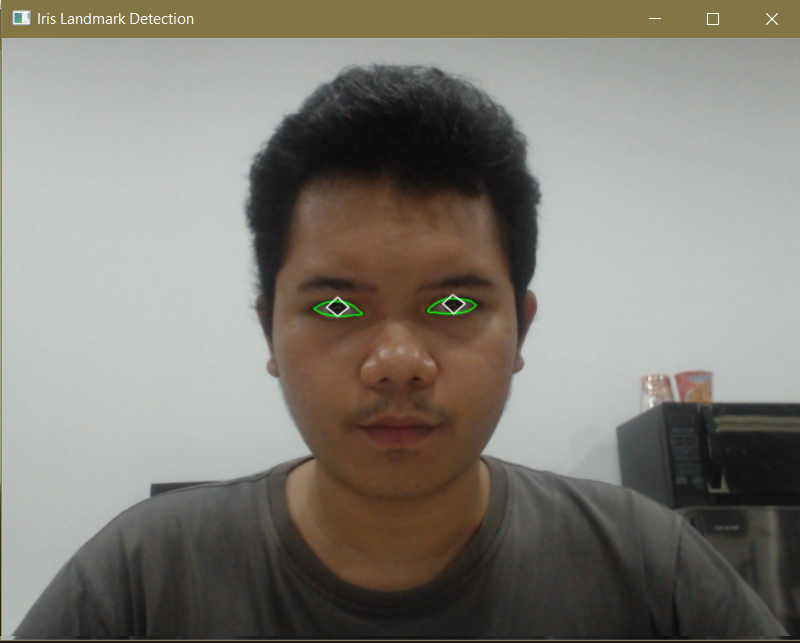
\includegraphics[width=0.15\textwidth]{gambar/bab4/131.png}
    %\caption{70 sentimeter}
    \label{fig:imagecc}}

  \caption{Variasi Pencahayaan}
  \label{fig:Variasi Pencahayaan}
\end{figure}

\begin{table}[ht]
  \caption{Pengujian Model dengan Pencahayaan 35 Lux}
  \label{tb:lux35} 
  \centering
  \begin{tabular}{|l|c|c|}
  \hline
  \rowcolor[HTML]{C0C0C0} 
  \textbf{Kelas} &  \multicolumn{1}{c|}{\textbf{\begin{tabular}[c]{@{}c@{}}Persentase \\ Keberhasilan\end{tabular}}} & \multicolumn{1}{c|}{\textbf{\begin{tabular}[c]{@{}c@{}}Persentase\\ Ketidakberhasilan\end{tabular}}} \\ \hline
  Kanan                                                                                                                                                                             & 100\%                                                                                   & 0\%                                                                                         \\ \hline
  Kiri                                                                                                                                                                               & 100\%                                                                                   & 0\%                                                                                         \\ \hline
  Maju                                                                                                                                                                              & 90\%                                                                                    & 10\%                                                                                        \\ \hline
  Mundur                                                                         & 93.33\%                                                                                 & 6.67\%                                                                                      \\ \hline
  Stop                                                                                          & 100\%                                                                                   & 0\%                                                                                         \\ \hline
\end{tabular}
\end{table}

\begin{table}[ht]
  \caption{Pengujian Model dengan Pencahayaan 55 Lux}
  \label{tb:lux55} 
  \centering
  \begin{tabular}{|l|c|c|}
  \hline
  \rowcolor[HTML]{C0C0C0} 
  \textbf{Kelas} &  \multicolumn{1}{c|}{\textbf{\begin{tabular}[c]{@{}c@{}}Persentase \\ Keberhasilan\end{tabular}}} & \multicolumn{1}{c|}{\textbf{\begin{tabular}[c]{@{}c@{}}Persentase\\ Ketidakberhasilan\end{tabular}}} \\ \hline
  Kanan                                                                                                                                                                             & 100\%                                                                                   & 0\%                                                                                         \\ \hline
  Kiri                                                                                                                                                                               & 100\%                                                                                   & 0\%                                                                                         \\ \hline
  Maju                                                                                                                                                                              & 96.67\%                                                                                    & 3.33\%                                                                                        \\ \hline
  Mundur                                                                         & 93.33\%                                                                                 & 6.67\%                                                                                      \\ \hline
  Stop                                                                                          & 100\%                                                                                   & 0\%                                                                                         \\ \hline
\end{tabular}
\end{table}

\begin{table}[H]
  \caption{Pengujian Model dengan Pencahayaan 131 Lux}
  \label{tb:lux131} 
  \centering
  \begin{tabular}{|l|c|c|}
  \hline
  \rowcolor[HTML]{C0C0C0} 
  \textbf{Kelas} &  \multicolumn{1}{c|}{\textbf{\begin{tabular}[c]{@{}c@{}}Persentase \\ Keberhasilan\end{tabular}}} & \multicolumn{1}{c|}{\textbf{\begin{tabular}[c]{@{}c@{}}Persentase\\ Ketidakberhasilan\end{tabular}}} \\ \hline
  Kanan                                                                                                                                                                             & 100\%                                                                                   & 0\%                                                                                         \\ \hline
  Kiri                                                                                                                                                                               & 100\%                                                                                   & 0\%                                                                                         \\ \hline
  Maju                                                                                                                                                                              & 100\%                                                                                    & 0\%                                                                                        \\ \hline
  Mundur                                                                         & 100\%                                                                                 & 0\%                                                                                      \\ \hline
  Stop                                                                                          & 100\%                                                                                   & 0\%                                                                                         \\ \hline
\end{tabular}
\end{table}

\subsection{Pengujian Performa \emph{Frame Per Second} (FPS) pada Sistem Kontrol Kursi Roda}

Pengujian performa \emph{Frame Per Second} (FPS) bertujuan untuk mengevaluasi kecepatan sistem dalam memproses pose mata secara real-time untuk mengontrol kursi roda. FPS merupakan indikator penting dalam menilai kelancaran dan responsivitas sistem, terutama dalam aplikasi yang memerlukan deteksi pose dan pengambilan keputusan yang cepat. Hasil pengujian FPS pada laptop dan NUC dapat dilihat pada Tabel \ref{tb:fps}.

\begin{table}[H]
  \caption{Hasil Performa FPS pada Laptop dan NUC}
  \label{tb:fps}
  \centering
  \begin{tabular}{|l|c|c|}
  \hline
  \rowcolor[HTML]{C0C0C0} 
  \textbf{Kelas} & \textbf{Rata-rata FPS Laptop} & \textbf{Rata-rata FPS NUC} \\ \hline
  Kanan           & 12.745              & 10.567           \\ \hline
  Kiri           & 12.635              & 10.617            \\ \hline
  Maju           & 13.078              & 10.068           \\ \hline
  Mundur           & 13.507              & 9.734           \\ \hline
  Stop           & 12.580              & 10.127            \\ \hline
  \end{tabular}
\end{table}

\subsection{Pengujian Inference Time pada Model dan Response Time pada Motor Kursi Roda}

Pengujian \emph{Inference Time} pada model dan \emph{Response Time} pada motor kursi roda bertujuan untuk mengevaluasi seberapa cepat sistem kontrol kursi roda berbasis pose mata dapat merespons perintah dari pengguna. \emph{Inference Time} mengukur waktu yang dibutuhkan oleh model untuk mendeteksi dan mengklasifikasikan pose mata, sementara \emph{Response Time} mengukur waktu yang diperlukan motor kursi roda untuk mulai bergerak setelah menerima sinyal dari model. Hasil pengujian waktu dari \emph{Inference Time} dan \emph{Response Time} dapat dilihat pada Tabel \ref{tb:response}.

\begin{table}[H]
  \caption{Hasil Pengujian Inference Time dan Response Time}
  \label{tb:response}
  \centering
  \begin{tabular}{|l|c|c|}
  \hline
  \rowcolor[HTML]{C0C0C0} 
  \textbf{Kelas} &  \multicolumn{1}{c|}{\textbf{\begin{tabular}[c]{@{}c@{}}Rata-rata \\ \emph{Inference Time} (s)\end{tabular}}} & \multicolumn{1}{c|}{\textbf{\begin{tabular}[c]{@{}c@{}}Rata-rata\\ \emph{Response Time} (s)\end{tabular}}} \\ \hline
  Kanan           & 0.0626             & 0.2328           \\ \hline
  Kiri           & 0.0640              & 0.0933            \\ \hline
  Maju           & 0.0656               & 0.4337           \\ \hline
  Mundur           & 0.0637              & 0.1409           \\ \hline
  Stop           & 0.0666              & 0.4318            \\ \hline
  \end{tabular}
\end{table}

\subsection{Pengujian Kestabilan pada Motor Kursi Roda}

Pengujian kestabilan pada motor kursi roda bertujuan untuk memastikan bahwa waktu output yang dijalankan oleh motor tetap stabil untuk setiap input yang diberikan oleh pengguna melalui sistem kontrol pose mata. Pengujian ini melibatkan pengukuran waktu yang dibutuhkan oleh motor untuk merespons setiap perintah pose mata dan memastikan bahwa waktu respons tersebut tetap konsisten di berbagai kondisi input. Hasil pengujian kestabilan motor dapat dilihat pada Tabel \ref{tb:stabil}.

\begin{table}[H]
  \caption{Hasil Pengujian Kestabilan Motor}
  \label{tb:stabil}
  \centering
  \begin{tabular}{|l|c|c|}
  \hline
  \rowcolor[HTML]{C0C0C0} 
  \textbf{Kelas} &  \multicolumn{1}{c|}{\textbf{\begin{tabular}[c]{@{}c@{}}Rata-rata \\ Lama Motor Berjalan (s)\end{tabular}}} \\ \hline
  Kanan          & 6.013                        \\ \hline
  Kiri           & 6.469                          \\ \hline
  Maju           & 6.532                         \\ \hline
  Mundur         & 6.863                         \\ \hline
  Stop           & 4.933                          \\ \hline
  \end{tabular}
\end{table}
% Ubah judul dan label berikut sesuai dengan yang diinginkan.
\section{Kesimpulan}
\label{sec:kesimpulan}

% Ubah paragraf-paragraf pada bagian ini sesuai dengan yang diinginkan.

Berdasarkan hasil pengujian yang telah dilakukan dan dianalisa pada bab sebelumnya, didapatkan beberapa kesimpulan sebagai berikut:

\begin{enumerate}

  \item Penelitian ini berhasil mengembangkan sistem kontrol kursi roda berbasis gestur mata menggunakan MediaPipe dan Intel NUC. Sistem ini mampu mengenali gerakan mata dengan tingkat akurasi tinggi dan menerjemahkannya menjadi perintah untuk mengontrol kursi roda. Sistem ini menawarkan solusi inovatif bagi pasien ALS yang hanya dapat menggerakkan mata.

  \item Model klasifikasi yang digunakan menunjukkan kinerja yang sangat baik berdasarkan hasil evaluasi confusion matrix. Model dapat mengenali berbagai gerakan mata dengan cepat dan konsisten, memastikan kontrol kursi roda yang andal.

  \item Model tetap memiliki performa yang stabil pada jarak 30 hingga 90 cm. Pada jarak 30 dan 50 cm, model memiliki akurasi tertinggi yaitu 100\%. Model menunjukkan bahwa semakin dekat jarak mata dengan kamera, semakin tinggi akurasi yang dihasilkan.

  \item Model memiliki kinerja yang cukup baik di berbagai tingkat pencahayaan, dengan akurasi tertinggi 100\% pada pencahayaan 131 Lux. Hal ini menunjukkan bahwa cahaya memiliki pengaruh yang signifikan terhadap akurasi model, dengan peningkatan akurasi pada pencahayaan yang lebih tinggi.

  \item Pengujian performa FPS menunjukkan bahwa sistem dapat mempertahankan FPS yang stabil pada laptop (10,415 - 13,972 FPS) dan Intel NUC (8,405 - 12,448 FPS). Variasi ini memastikan bahwa sistem tetap responsif terhadap gerakan mata pengguna.
  
  \item Waktu respons rata-rata motor untuk perintah "Kanan," "Kiri," dan "Mundur" di bawah 0,25 detik, menunjukkan sistem yang responsif. Sedangkan untuk perintah "Maju" adalah 0,4337 detik dan untuk perintah "Stop" adalah 0,4318, menunjukkan waktu respons yang lebih tinggi karena perintah tersebut memerlukan waktu yang lebih lama untuk dieksekusi.
  
  \item Motor kursi roda memiliki waktu output yang konsisten di setiap kelas perintah, dengan variabilitas yang relatif sempit dengan nilai standar deviasi untuk kelas "Kanan" sebesar 0,408, kelas "Kiri" sebesar 0,371, kelas "Maju" sebesar 0,117, kelas "Mundur" sebesar 0,156, dan kelas "Stop" sebesar 0,361. Di antara semua kelas perintah, kelas maju memiliki nilai yang paling stabil, menunjukkan keandalan sistem dalam memberikan respons stabil dan konsisten saat perintah maju diberikan.

\end{enumerate}
% Ucapan terima kasih jika ada
\section{Ucapan Terima Kasih}
\label{sec:ucapanterimakasih}

Penulis mengucapkan terima kasih kepada Kementerian Riset, Teknologi, dan Pendidikan Tinggi Republik Indonesia atas \lipsum[1]

% Menampilkan daftar pustaka dengan format IEEE
\bibliographystyle{IEEEtranN}
\bibliography{pustaka/pustaka.bib}

% Menyeimbangkan bagian akhir di kedua kolom
\balance

\end{document}